\FloatBarrier
\begin{figure}[!htbp]
\centering
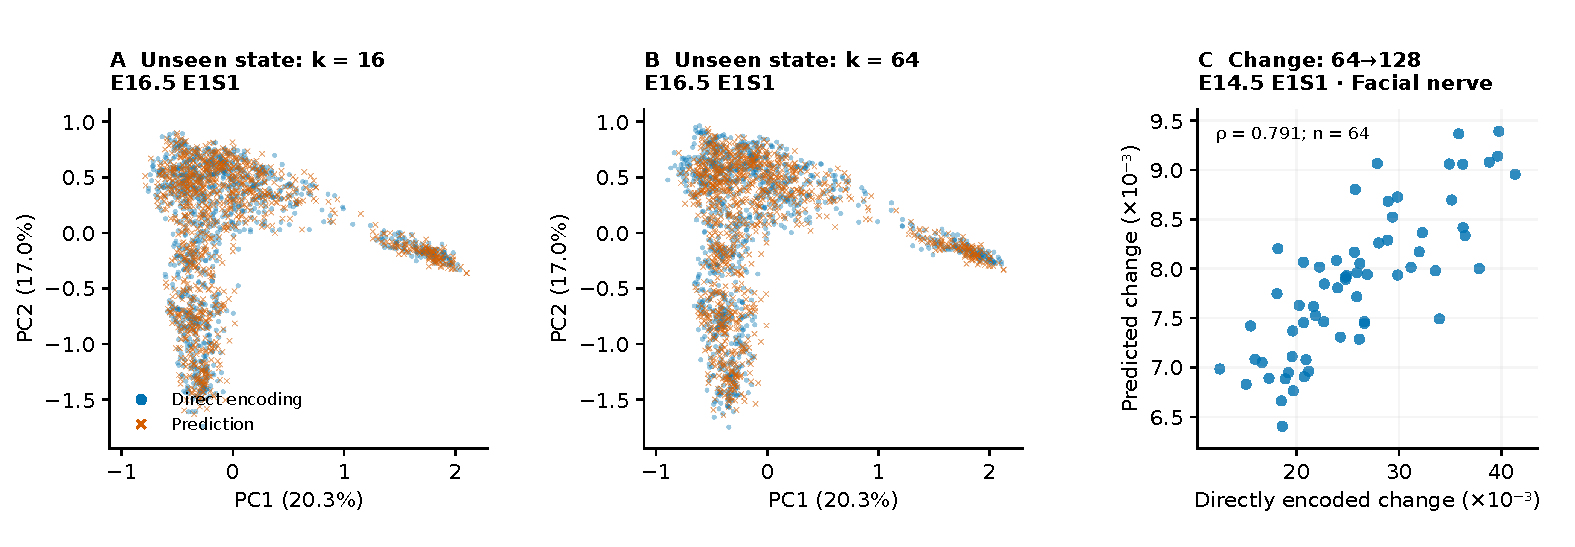
\includegraphics[width=\linewidth]{figures/unseen_states_and_response.pdf}
\caption{\textbf{Illustrative unseen-state predictions and response correlation in source-section cases.} \textbf{A,B}, Direct encodings and predictions at unseen granularities 16 and 64 for 1,024 matched E16.5 E1S1 positions, using a shared PCA basis fitted on direct encodings at nine granularities. Full-dimensional $R^2$ is 0.941 and 0.876. \textbf{C}, Predicted versus directly encoded change over $64\to128$ in E14.5 E1S1 Facial nerve. Points show all 64 matched locations; axes report RMS representation change. Both sections belong to the training set. All predictions start from $e_8$; 16 and 64 are absent from granularity supervision. Held-out prediction and response summaries are shown separately in Figures~\ref{fig:generalization-summary} and~\ref{fig:heldout-response-ordering}.}
\label{fig:scale-continuum}
\end{figure}
\FloatBarrier
